\scanpage{3}
$X$ courbe non singulière

$\mathcal E$ anneau des classes de faisceaux cohérents mod les
$(\underline F)-(\underline F')-(\underline F'')$, \unsure{rel les|relts}
\inserted{\unsure{i.e.} suite exacte $0\to F'\to F\to F''\to0$.}
\unsure{aux} $F$ à support \uline{discret}

$\mathcal E_0$ noyau de l'augmentation (rang)

$D$ sous-anneau engendré par les faisceaux \deleted{\unsure{définis}} du type $k_x$

$D=$ groupe des diviseurs. $*$ C'est l'\uline{annulateur de $\mathcal E_0$}, donc un idéal

$N$ sous-groupe de $\mathcal E$ engendré par les
$(\underline F)-(\underline F')-(\underline F'')$

$D\cap N$ \deleted{\illegible{1}} diviseurs ``\unsure{f}-équivalents'' à $0$,
\deleted{\illegible{1}}\inserted{identiques à}

$L$ groupe des diviseurs équivalents à $0$

$\Phi$ sous-algèbre de $\mathcal E$ engendrée par les \deleted{\unsure{de}} faisceaux loc. libres

$\simeq$ algèbre des classes de fibrés vectoriels, on a

$\Phi_N$ \unsure{Quotient} de $\Phi$ par le sous-groupe ($=$ idéal) engendré par les
$c(E)-c(E')-c(E'')$
\[
*\quad \mathcal E=\Phi+D\qquad \Phi\cap D=0
\]
\[
*\quad \mathcal E/N\simeq\Phi/\Phi_N\simeq \unsure{Z|\mathbb Z}+\unsure{\mathfrak P|\mathfrak D}^{(1)}
\]
\deleted{$*\quad\unsure{D_f\subset D_0}$\quad \unsure{diviseurs} \illegible{2}\\
\unsure{défini} \illegible{2}}

\uline{Proposition} $N$ est engendré par les $c(E)-c(E')-c(E'')$, où
$0\to E'\to E\to E''\to0$ est une suite exacte de fibrés \uline{vectoriels}, et
les $c(E)-c(F)-c(\underline O_x(E)/f\underline O_x(F))$, où $E$ et $F$ sont des fibrés
\uline{linéaires} et $f:F\to E$ un \unsure{hom} non nul,
\unsure{i.e.} $f\in H^0(X,\underline O_x(F^*\otimes E))$.

Ces derniers éléments sont aussi ceux de la forme
$\lambda(D+D')-\lambda(D')-D$ \deleted{\illegible{1}}
($D$ et $D'$ diviseurs\deleted{\illegible{1}}),
$\lambda(\Delta)$ est la classe du faisceau associé au fibré vectoriel associé au diviseur $\Delta$.
On peut se borner à $D\geq0$

\margin{$(1)$ $\unsure{Z|\mathbb Z}+\unsure{\mathfrak P|\mathfrak D}\to\mathcal E/N$ fait correspondre à $(1,0)$ la classe de
$\underline O_x$, et sur $\unsure{\mathfrak P|\mathfrak D}$ se définit par passage au quotient de l'inclusion
$D\subset\mathcal E$}

\margin{\unsure{LINEN TYPEWRITER}\quad
\figure{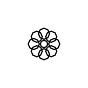
\begin{tikzpicture}[scale=.13]
\foreach \a in {0,45,...,315}{\draw (\a:1) circle (.54);}
\draw (0,0) circle (.36);
\end{tikzpicture}}\quad \unsure{ARGENTINA}}

\margin{2}
